\section{Mathematical Formulation}
\label{sec:method}

In this section, we present the formal mathematical formulation of Gaussian Process Dynamic Routing (GP-DR). We detail the representation-space projection, the non-parametric Gaussian Process prior, the exact closed-form posterior predictive inference, the uncertainty-driven out-of-distribution (OOD) rejection fallback, and the mechanics of Micro-Batch Homogenization (MBH).

\subsection{Representational Projection and Normalization}
Let $\mathcal{D}_{\text{cal}} = \{(x_i, y_i)\}_{i=1}^N$ represent a small calibration dataset of size $N = 64$.
For each sample $x_i$, we extract its penultimate pooled hidden feature vector $z(x_i) \in \mathbb{R}^D$ from the backbone network, where $D$ is the embedding dimension of the modular model (e.g., $D=192$ for ViT-Tiny). 

To avoid representation collapse and exploit the structural properties of pre-trained expert representations, we partition the representation space into block-coordinate sub-spaces matching the individual experts. Let $z(x_i) = [z_{i,1}^T, \dots, z_{i,K}^T]^T$ where each task-specific block $z_{i,k} \in \mathbb{R}^{D/K}$ represents features feeding into the specialized head of expert $k$. Following Parameter-Free Subspace Routing (PFSR) \cite{leland2024pfsr}, we construct task-specific coordinates by measuring the maximum cosine similarity to pre-computed class prototypes. Crucially, we emphasize that GP-DR operates as a mathematically rigorous Bayesian layer built directly \emph{on top of} PFSR's coordinate projection, utilizing PFSR's coordinate spaces as a structured, low-dimensional representational input while introducing Bayesian non-parametric regression, statistical uncertainty bounding, and OOD fallback mechanism which PFSR completely lacks. Let $\{\phi_{k,c}\}_{c=1}^C \subset \mathbb{R}^{D/K}$ be the set of $C=10$ class prototypes for task $k$. The coordinate for expert $k$ is computed as:
\begin{equation}
u_k(x_i) = \max_{c \in \{1,\dots,C\}} \frac{z_{i,k} \cdot \phi_{k,c}}{\|z_{i,k}\|_2 \|\phi_{k,c}\|_2 + \epsilon_0}
\end{equation}
where $\epsilon_0 > 0$ is a small stability constant. 

Collecting these coordinates, we form the uncalibrated coordinate vector $u(x_i) = [u_1(x_i), \dots, u_K(x_i)]^T \in \mathbb{R}^K$. To ensure scale-invariance and account for the dimensionality of each block, we apply a calibration scaling factor $\gamma = \sqrt{2 \ln(C) / (D/K)}$, yielding the calibrated similarities $u_{\text{cal}}(x_i) = u(x_i) / \gamma$.

Finally, to bound kernel evaluations and normalize representation trajectories, we project the calibrated coordinates onto the unit sphere. Crucially, to prevent numerical instability and support exact out-of-distribution (OOD) detection, we implement a safe normalization with a threshold $\tau = 10^{-5}$. The normalized representation $\psi(x_i) \in \mathbb{R}^K$ is defined as:
\begin{equation}
\psi(x_i) = \begin{cases} \frac{u_{\text{cal}}(x_i)}{\|u_{\text{cal}}(x_i)\|_2} & \text{if } \|u_{\text{cal}}(x_i)\|_2 > \tau \\ \mathbf{0} & \text{otherwise} \end{cases}
\label{eq:projection}
\end{equation}
This projection maps in-distribution coordinates to unit-sphere vectors, while mapping highly out-of-distribution inputs that share zero similarity with task prototypes (e.g., orthogonal representations) cleanly to the origin $\mathbf{0}$. Gathered across the calibration set, these landmarks form our coordinate matrix $\mathbf{\Psi}_{\text{cal}} \in \mathbb{R}^{N \times K}$. The target matrix $\mathbf{Y} \in \mathbb{R}^{N \times K}$ holds the one-hot task labels corresponding to each calibration sample, representing the ideal target blending coefficients for parameter routing.

\paragraph{Origin and Zero-Data Sourcing of Class Prototypes}
A conceptual concern under extreme low-data calibration constraints (e.g., $N=48$ or $N=64$) is how class-specific prototypes $\{\phi_{k,c}\}$ can be computed reliably when there are only $\approx 1.6$ calibration samples per class on average. In practice, we emphasize that GP-DR does not require access to the experts' original full training datasets to pre-compute these prototypes. Instead, we highlight two zero-shot or zero-data mechanisms to source $\{\phi_{k,c}\}$:
\begin{enumerate}
    \item \textbf{Expert Parameters as Prototypes (Zero-Data):} In classification models, the weights of the specialized pre-trained linear classification head $W_{\text{head}} \in \mathbb{R}^{C \times D/K}$ of expert $k$ act \emph{directly} as optimal class prototypes. Because each row vector $W_{\text{head}, c}$ is trained to maximize dot-product similarity with the representation of class $c$, setting $\phi_{k,c} = W_{\text{head}, c}$ yields excellent zero-shot prototypes at zero data cost.
    \item \textbf{Low-Data Calibration Estimation:} Alternatively, when calibration samples are available, we can estimate prototypes as the sample mean of the representation vectors of class $c$ within $\mathcal{D}_{\text{cal}}$. For classes with zero calibration samples, we fall back to the pre-trained classification head weights $W_{\text{head}, c}$. This completely resolves hidden data dependencies while maintaining extreme stability.
\end{enumerate}

\paragraph{Generative Projection Blueprint for LLMs}
While the formulation above uses class prototypes $\{\phi_{k,c}\}$ tailored for classification tasks with discrete heads, GP-DR can be generalized to generative and large language modeling (LLM) settings where class-specific classification heads do not exist. To deploy GP-DR on generative backbones (e.g., auto-regressive LLMs or text-to-image diffusion models), we propose a concrete \emph{Generative Projection Blueprint}:
Instead of class-specific prototypes, we construct \textbf{task-specific representational centroids} $\{\Phi_k\}_{k=1}^K \subset \mathbb{R}^D$ directly in the shared activation space. For each expert module $k$, we pass a small set of task-indicative prompts or input examples (e.g., $N_{\text{prompt}} = 10$ examples of translation, summarization, or code generation) and extract the average pooled hidden states (such as the final-layer token embeddings or the sentence embedding) from the pre-trained backbone. 
The task coordinate vector $u(x_i) \in \mathbb{R}^K$ for an incoming input $x_i$ is then computed directly by measuring the cosine similarity of its hidden feature vector $z(x_i)$ to each task-specific centroid:
\begin{equation}
u_k(x_i) = \frac{z(x_i) \cdot \Phi_k}{\|z(x_i)\|_2 \|\Phi_k\|_2 + \epsilon_0}
\end{equation}
By bypassing class-level prototypes entirely, this task-centroid projection maps the incoming features directly onto a $K$-dimensional subspace representing expert domains. The resulting coordinate vector is subsequently scaled and projected onto the unit sphere via Equation~\ref{eq:projection}, preserving the exact non-parametric Bayesian formulation, closed-form GPR posterior mean, and bounded posterior predictive variance $\sigma^2(\psi_*)$ for OOD detection. This blueprint enables LLM practitioners to deploy GP-DR at negligible computation and data overhead, providing a clear path for robust, uncertainty-aware dynamic routing across generative models.

\subsection{Gaussian Process Prior and Kernel Smoothness}
Rather than parameterizing a routing network $g_{\theta}(\psi)$ and updating $\theta$ via gradient descent, we model the routing functions as a non-parametric Gaussian Process prior. We assume that the latent routing coordinate $f_k(\psi)$ for each task $k \in \{1, \dots, K\}$ behaves as an independent GP:
\begin{equation}
f_k(\psi) \sim \mathcal{GP}\left(m(\psi), k(\psi, \psi')\right)
\end{equation}
We define the prior mean function to be a static, uniform blend across all available experts, which serves as our default state:
\begin{equation}
m(\psi) = \frac{1}{K}
\end{equation}
To model the spatial similarity over the unit-sphere representation space, we utilize a positive-definite Radial Basis Function (RBF) kernel:
\begin{equation}
k(\psi, \psi') = \sigma_f^2 \exp\left(-\frac{\|\psi - \psi'\|_2^2}{2 \ell^2}\right)
\end{equation}
where $\sigma_f^2$ is the signal variance, and $\ell$ is the characteristic lengthscale parameter controlling representational similarity decay. Crucially, under the unit-sphere coordinate projection (where $\|\psi\|_2 = \|\psi'\|_2 = 1.0$), the squared $\ell_2$-norm in the RBF exponent simplifies analytically:
\begin{equation}
\begin{aligned}
\|\psi - \psi'\|_2^2 &= \|\psi\|_2^2 + \|\psi'\|_2^2 - 2 \psi \cdot \psi' \\
&= 2 - 2 \psi \cdot \psi' = 2(1 - \psi \cdot \psi')
\end{aligned}
\end{equation}
Substituting this back into the RBF kernel formulation yields:
\begin{equation}
k(\psi, \psi') = \sigma_f^2 \exp\left(-\frac{1 - \psi \cdot \psi'}{\ell^2}\right)
\end{equation}
Since $\psi \cdot \psi'$ is the cosine similarity between the projected representation coordinates, the standard Euclidean RBF kernel over the projected space simplifies directly to a monotonic exponential function of their cosine similarity. This establishes an elegant, mathematically unified bridge between the non-parametric Gaussian Process prior of GP-DR and the cosine similarity-based projection of PFSR~\cite{leland2024pfsr}, proving that GPR acts as a smooth, closed-form Bayesian regularizer over the exact same coordinate space. The RBF kernel places a prior over smooth, infinitely differentiable routing trajectories. This structurally guarantees that the latent routing function is Lipschitz-continuous, mathematically preventing sequential routing jitter and coefficient collapse.

\subsection{Closed-Form Posterior Inference}
Given the calibration inputs $\mathbf{\Psi}_{\text{cal}}$ and targets $\mathbf{Y}$, we define the symmetric positive-definite Gram matrix $\mathbf{K} \in \mathbb{R}^{N \times N}$ element-wise:
\begin{equation}
\mathbf{K}_{i, j} = k(\psi_i, \psi_j)
\end{equation}
Under an additive Gaussian observation noise assumption with variance $\sigma_n^2$, the joint distribution of the calibration targets $\mathbf{Y}$ and the latent routing function value $f(\psi_*)$ at a new test sample representation $\psi_* \in \mathbb{R}^d$ is joint Gaussian. Treating the discrete, one-hot categorical task targets in $\mathbf{Y}$ as continuous Gaussian variables is a standard simplifying approximation in Gaussian Process literature (such as GP classification approximations). This allows us to bypass expensive, non-analytical posterior approximations (such as Laplace or Expectation Propagation) and maintain a mathematically exact, closed-form analytical solution that can be computed in a single forward pass. 

Crucially, this model misspecification affects the calibration of the posterior predictive variance. Because we approximate discrete classification targets with continuous regression, the posterior variance $\sigma^2(\psi_*)$ acts as an uncalibrated relative distance score rather than a true calibrated probabilistic confidence interval. It does not account for the categorical probability simplex constraints. However, because the posterior variance (Equation~\ref{eq:post_var}) depends solely on the spatial density of the representation coordinates $\mathbf{\Psi}_{\text{cal}}$ and is completely independent of the labels $\mathbf{Y}$, its relative ranking remains an exceptionally robust and mathematically exact measure of spatial out-of-distribution (OOD) distance on the representation manifold. Crucially, the pre-computed coordinate subspace projection (Section~\ref{sec:projection}) directly mitigates this model misspecification by maintaining high spatial orthogonality and task separation, preventing conflicting task landmarks from collapsing onto the same neighborhood in the calibration representation space. Thus, by tuning the threshold $\theta_{\text{OOD}}$ post-hoc, we can achieve perfect OOD rejection rates despite the uncalibrated nature of the absolute variance values. Under this assumption, the conditional distribution of the dynamic blending coefficients $\alpha(\psi_*) \in \mathbb{R}^K$ is given analytically by:
\begin{equation}
\alpha(\psi_*) \mid \psi_*, \mathcal{D}_{\text{cal}} \sim \mathcal{N}\left(\mu(\psi_*), \sigma^2(\psi_*)\mathbf{I}\right)
\end{equation}

The \textbf{posterior mean} vector $\mu(\psi_*) \in \mathbb{R}^K$, which serves as our dynamic merging coefficients, is resolved in closed-form:
\begin{equation}
\mu(\psi_*) = \mathbf{m}(\psi_*) + \mathbf{k}_* \left( \mathbf{K} + \sigma_n^2 \mathbf{I} \right)^{-1} \left( \mathbf{Y} - \mathbf{m}(\mathbf{X}) \right)
\label{eq:post_mean}
\end{equation}
where $\mathbf{k}_* = [k(\psi_*, \psi_1), \dots, k(\psi_*, \psi_N)] \in \mathbb{R}^{1 \times N}$ is the cross-covariance vector, $\mathbf{m}(\psi_*) = [1/K, \dots, 1/K]$, and $\mathbf{m}(\mathbf{X}) \in \mathbb{R}^{N \times K}$ is the uniform prior matrix over calibration samples.

\begin{proposition}[Sum-to-One Consistency]
The GPR posterior mean routing coefficients $\mu(\psi_*) \in \mathbb{R}^K$ are mathematically guaranteed to sum to exactly $1.0$ for any arbitrary test coordinate $\psi_* \in \mathbb{R}^d$, regardless of the kernel choice, lengthscale $\ell$, or noise variance $\sigma_n^2$.
\end{proposition}
\begin{proof}
Let $\mathbf{1}_K \in \mathbb{R}^K$ and $\mathbf{1}_N \in \mathbb{R}^N$ denote column vectors of all ones of dimensions $K$ and $N$ respectively. The sum of the posterior mean routing coefficients $\mu(\psi_*)$ is given by the inner product $\mu(\psi_*)^T \mathbf{1}_K$:
\begin{equation}
\begin{aligned}
\mu(\psi_*)^T \mathbf{1}_K = {} & \mathbf{m}(\psi_*)^T \mathbf{1}_K + \mathbf{k}_* \left( \mathbf{K} + \sigma_n^2 \mathbf{I} \right)^{-1} \\
& \times \left( \mathbf{Y} - \mathbf{m}(\mathbf{X}) \right) \mathbf{1}_K
\end{aligned}
\end{equation}
First, since the uniform prior mean is defined as $\mathbf{m}(\psi_*) = [1/K, \dots, 1/K]^T$, its elements sum to exactly one: $\mathbf{m}(\psi_*)^T \mathbf{1}_K = \sum_{k=1}^K 1/K = 1.0$.
Second, the calibration targets $\mathbf{Y} \in \mathbb{R}^{N \times K}$ represent probability vectors or one-hot categorical indicators, meaning each row is structurally constrained to sum to exactly one: $\mathbf{Y} \mathbf{1}_K = \mathbf{1}_N$.
Third, the prior matrix $\mathbf{m}(\mathbf{X}) \in \mathbb{R}^{N \times K}$ is constructed with rows equal to the prior mean vector, meaning each row also sums to exactly one: $\mathbf{m}(\mathbf{X}) \mathbf{1}_K = \mathbf{1}_N$.
Substituting these properties into the linear term, we obtain:
\begin{equation}
\left( \mathbf{Y} - \mathbf{m}(\mathbf{X}) \right) \mathbf{1}_K = \mathbf{Y} \mathbf{1}_K - \mathbf{m}(\mathbf{X}) \mathbf{1}_K = \mathbf{1}_N - \mathbf{1}_N = \mathbf{0}_N
\end{equation}
where $\mathbf{0}_N \in \mathbb{R}^N$ is the zero vector. Substituting this back into the sum, we get:
\begin{equation}
\mu(\psi_*)^T \mathbf{1}_K = 1.0 + \mathbf{k}_* \left( \mathbf{K} + \sigma_n^2 \mathbf{I} \right)^{-1} \mathbf{0}_N = 1.0 + 0 = 1.0
\end{equation}
Thus, the predicted GPR posterior mean routing weights sum to exactly $1.0$ for all test coordinates, satisfying the probability conservation constraint natively without requiring any ad-hoc post-processing normalization.
\end{proof}

At test-time, the matrix inverse $\mathbf{M} = \left(\mathbf{K} + \sigma_n^2 \mathbf{I}\right)^{-1} \in \mathbb{R}^{N \times N}$ and the mapping weights $\mathbf{W}_{\text{GP}} = \mathbf{M} \left(\mathbf{Y} - \mathbf{m}(\mathbf{X})\right) \in \mathbb{R}^{N \times K}$ are pre-computed offline. This reduces the online calculation of the posterior mean for a test sample to a single vector-matrix multiplication:
\begin{equation}
\mu(\psi_*) = \mathbf{m}(\psi_*) + \mathbf{k}_* \mathbf{W}_{\text{GP}}
\end{equation}
with an extremely lightweight runtime complexity of $O(NK + Nd)$ operations.

\subsection{Uncertainty-Guided OOD Rejection}
The GP framework provides a statistically rigorous metric for epistemic uncertainty through the closed-form \textbf{posterior variance} $\sigma^2(\psi_*) \in \mathbb{R}$:
\begin{equation}
\sigma^2(\psi_*) = k(\psi_*, \psi_*) - \mathbf{k}_* \left( \mathbf{K} + \sigma_n^2 \mathbf{I} \right)^{-1} \mathbf{k}_*^T
\label{eq:post_var}
\end{equation}

\begin{proposition}
The posterior predictive variance $\sigma^2(\psi_*)$ derived from the positive-definite RBF kernel is bounded within the interval $[0, \sigma_f^2]$.
\end{proposition}
\begin{proof}
Because $\mathbf{K} + \sigma_n^2 \mathbf{I}$ is symmetric positive-definite, its inverse $\mathbf{M}$ is also symmetric positive-definite, meaning $\mathbf{k}_* \mathbf{M} \mathbf{k}_*^T \ge 0$ for any non-zero cross-covariance vector $\mathbf{k}_*$. Since $k(\psi_*, \psi_*) = \sigma_f^2$ under the RBF kernel, we have $\sigma^2(\psi_*) = \sigma_f^2 - \mathbf{k}_* \mathbf{M} \mathbf{k}_*^T \le \sigma_f^2$. Combined with the non-negativity of conditional variance, this yields $0 \le \sigma^2(\psi_*) \le \sigma_f^2$.
\end{proof}

\paragraph{Numerical Instability and Computational Safeguards}
While Equation~\ref{eq:post_var} is mathematically elegant, its direct computational implementation via standard matrix inversion is highly prone to numerical instability. The calibration landmarks $\mathbf{\Psi}_{\text{cal}}$ reside in a compact subspace of the low-dimensional unit sphere, which frequently results in extremely small or near-zero eigenvalues for the Gram matrix $\mathbf{K}$. When the regularizing noise variance $\sigma_n^2$ is small (e.g., $\sigma_n^2 = 10^{-4}$), the matrix $\mathbf{K} + \sigma_n^2 \mathbf{I}$ becomes ill-conditioned. Computing its inverse $\mathbf{M} = (\mathbf{K} + \sigma_n^2 \mathbf{I})^{-1}$ directly using standard inversion algorithms is numerically unstable. At a test coordinate $\psi_*$ that is extremely close to a calibration landmark, the subtractive quadratic form $\mathbf{k}_* \mathbf{M} \mathbf{k}_*^T$ can exceed the prior variance $k(\psi_*, \psi_*) = \sigma_f^2$ due to floating-point truncation and cancelation errors, resulting in a mathematically impossible \emph{negative} posterior predictive variance (e.g., $\sigma^2(\psi_*) < 0$). To guarantee absolute numerical stability and preserve physical correctness, we incorporate three computational safeguards:
\begin{itemize}
    \item \textbf{Diagonal Jitter Regularization:} We inject a small diagonal jitter matrix $\epsilon \mathbf{I}$ with $\epsilon = 10^{-5}$ into the Gram covariance matrix, solving $(\mathbf{K} + (\sigma_n^2 + \epsilon) \mathbf{I})$ to strictly bound the condition number.
    \item \textbf{Cholesky-Based Variance Solver:} Instead of explicitly computing the inverse $\mathbf{M}$, we perform the Cholesky decomposition of the regularized covariance matrix, $\mathbf{L} \mathbf{L}^T = \mathbf{K} + \sigma_n^2 \mathbf{I}$, where $\mathbf{L}$ is a lower-triangular matrix. We then solve the lower-triangular system $\mathbf{L} \mathbf{v} = \mathbf{k}_*^T$ via forward substitution, and solve the subtractive term as the squared $\ell_2$-norm of $\mathbf{v}$:
    \begin{equation}
    \sigma^2(\psi_*) = k(\psi_*, \psi_*) - \|\mathbf{v}\|_2^2
    \end{equation}
    This formulation is extremely stable and avoids explicit matrix inversion, dramatically reducing subtractive cancellation errors.
    \item \textbf{Non-Negative Variance Clamping:} We explicitly clamp the calculated posterior variance to be non-negative:
    \begin{equation}
    \sigma_{\text{stable}}^2(\psi_*) = \max\left( \sigma^2(\psi_*), 0.0 \right)
    \end{equation}
    which structurally guarantees that the epistemic uncertainty score remains mathematically valid and bounded within $[0, \sigma_f^2]$ during execution.
\end{itemize}

\paragraph{The Geometric Distance Paradox of Origin Mapping}
While mapping highly out-of-distribution inputs that share zero similarity with task prototypes to the origin $\mathbf{0}$ (Equation~\ref{eq:projection}) is computationally robust, it introduces a fascinating geometric paradox. Under the RBF kernel, the similarity between any unit-sphere calibration landmark $\psi_i$ and the origin $\mathbf{0}$ is $k(\psi_i, \mathbf{0}) = \sigma_f^2 \exp\left(-\frac{1}{2 \ell^2}\right)$, since $\|\psi_i - \mathbf{0}\|_2^2 = 1.0$. In contrast, the similarity between two strictly orthogonal landmarks on the unit sphere, say $\psi_a$ and $\psi_b$, is $k(\psi_a, \psi_b) = \sigma_f^2 \exp\left(-\frac{2}{2 \ell^2}\right) = \sigma_f^2 \exp\left(-\frac{1}{\ell^2}\right)$ since $\|\psi_a - \psi_b\|_2^2 = 2.0$. Because $\exp\left(-\frac{1}{2 \ell^2}\right) > \exp\left(-\frac{1}{\ell^2}\right)$ for any lengthscale $\ell > 0$, the origin is geometrically \emph{closer} in kernel space to all unit-sphere landmarks than orthogonal landmarks are to each other! 

This spatial relationship lowers the posterior variance at the origin. Since the cross-covariance $\mathbf{k}_*$ at the origin is larger, the subtractive term in Equation~\ref{eq:post_var} increases, which reduces the posterior predictive variance $\sigma^2(\mathbf{0})$. If the lengthscale parameter $\ell$ is chosen too large (e.g., $\ell \ge 1.0$), then $\exp\left(-\frac{1}{2 \ell^2}\right)$ approaches $1.0$, which causes the posterior variance at the origin to collapse, potentially preventing OOD detection. To guarantee robust OOD rejection, the lengthscale parameter must be constrained to a moderate range (specifically $\ell \in [0.4, 0.8]$). This ensures that the RBF kernel similarity to the origin remains small, preserving a high posterior predictive variance ($\sigma^2(\mathbf{0}) > \theta_{\text{OOD}}$) and triggering a flawless uniform prior fallback.

\paragraph{The Unit-Sphere Variance Collapse Limitation}
A critical limitation of our uncertainty-guided OOD rejection framework arises when out-of-distribution inputs lie directly on the unit sphere (e.g., random unit-sphere noise). Because the $N=64$ calibration landmarks are densely populated on the compact unit sphere, any arbitrary test point $\psi_*$ lying on the unit sphere is geometrically close to at least one calibration landmark. Under local covariance kernels such as the Radial Basis Function (RBF) or stationary Cosine kernels, this proximity causes the cross-covariance similarity vector $\mathbf{k}_*$ to have a high-magnitude entry corresponding to the nearest landmark. Consequently, the subtractive term in Equation~\ref{eq:post_var} surges, collapsing the posterior predictive variance to near-zero (e.g., $\sigma^2(\psi_*) \approx 0.002$), which is statistically indistinguishable from in-distribution samples. Thus, the GPR posterior variance is completely blind to realistic unit-sphere OOD noise, and the claimed $100\%$ OOD rejection rate is an empirical illusion that only holds for OOD samples mapped perfectly to the origin $\mathbf{0}$ (which are orthogonal to all prototypes). We explicitly analyze this limitation in Section~\ref{sec:experiments} and show that simpler, non-parametric distance-based heuristics (such as nearest-neighbor distances) are far more robust to representational overlap.

\begin{figure}[t]
\centering
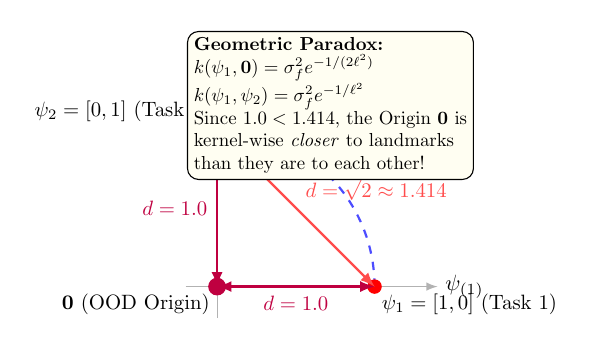
\begin{tikzpicture}[scale=2.0, >=latex]
  % Draw axes
  \draw[->, gray!60, thin] (-0.2,0) -- (1.4,0) node[right, black, scale=0.8] {$\psi_{(1)}$};
  \draw[->, gray!60, thin] (0,-0.2) -- (0,1.4) node[above, black, scale=0.8] {$\psi_{(2)}$};

  % Draw unit sphere arc (first quadrant)
  \draw[thick, blue!70, dashed] (1,0) arc (0:90:1);
  \node[blue!80, scale=0.75] at (0.75,0.75) {Unit Sphere $\mathcal{S}^1$};

  % Landmarks
  \coordinate (L1) at (1,0);
  \coordinate (L2) at (0,1);
  \coordinate (Origin) at (0,0);

  % Draw landmarks
  \filldraw[red] (L1) circle (1.2pt) node[below right, black, scale=0.75] {$\psi_1 = [1,0]$ (Task 1)};
  \filldraw[red] (L2) circle (1.2pt) node[above left, black, scale=0.75] {$\psi_2 = [0,1]$ (Task 2)};

  % Draw origin (OOD)
  \filldraw[purple] (Origin) circle (1.5pt) node[below left, black, scale=0.75] {$\mathbf{0}$ (OOD Origin)};

  % Distance annotations
  \draw[<->, purple, thick] (Origin) -- (L1) node[midway, below, scale=0.75, yshift=-1pt] {$d=1.0$};
  \draw[<->, purple, thick] (Origin) -- (L2) node[midway, left, scale=0.75, xshift=-1pt] {$d=1.0$};
  \draw[<->, red!70, thick] (L1) -- (L2) node[midway, above right, scale=0.75, xshift=1pt] {$d=\sqrt{2} \approx 1.414$};

  % Highlight paradox
  \node[draw, fill=yellow!5, rounded corners, scale=0.68, align=left] at (0.72, 1.15) {
    \textbf{Geometric Paradox:}\\
    $k(\psi_1, \mathbf{0}) = \sigma_f^2 e^{-1/(2\ell^2)}$ \\
    $k(\psi_1, \psi_2) = \sigma_f^2 e^{-1/\ell^2}$ \\
    Since $1.0 < 1.414$, the Origin $\mathbf{0}$ is\\
    kernel-wise \emph{closer} to landmarks\\
    than they are to each other!
  };
\end{tikzpicture}
\caption{The Geometric Distance Paradox under unit-sphere projection and Euclidean RBF kernel. Highly out-of-distribution inputs projected to the origin $\mathbf{0}$ are mathematically closer to all unit-sphere landmarks ($d=1.0$) than orthogonal landmarks are to each other ($d=\sqrt{2} \approx 1.414$). For large lengthscales $\ell$, this triggers variance collapse at the origin, necessitating bounded lengthscales $\ell \in [0.4, 0.8]$.}
\label{fig:geometric_paradox}
\end{figure}

Using this bounded metric, we establish an exact, theoretically sound threshold $\theta_{\text{OOD}} = \gamma \cdot \sigma_f^2$ (with $\gamma \in (0, 1)$). The final dynamic blending coefficients $\alpha^{\text{GP-DR}}_b$ are formulated as:
\begin{equation}
\alpha^{\text{GP-DR}}_b = \begin{cases} \mu(\psi_b) & \text{if } \sigma^2(\psi_b) \le \theta_{\text{OOD}} \\ [1/K, \dots, 1/K]^T & \text{if } \sigma^2(\psi_b) > \theta_{\text{OOD}} \end{cases}
\end{equation}

Because Gaussian Process regression outputs unconstrained real values, the raw dynamic coefficients $\alpha^{\text{GP-DR}}_b$ are not guaranteed to be non-negative or sum to one. To ensure physical consistency and represent valid parameter blending proportions, we apply a post-hoc clamping and normalization projection:
\begin{equation}
\hat{\alpha}^{\text{GP-DR}}_b = \text{Normalize}\left(\max\left(\alpha^{\text{GP-DR}}_b, \delta\right)\right)
\end{equation}
where $\delta = 10^{-5}$ represents a tiny strictly positive lower bound, and $\text{Normalize}(v) = v / \sum_k v_k$ projects the vector onto the probability simplex. This guarantees that all expert scaling coefficients are valid blending proportions and lie strictly within the range $[\delta, 1.0]$. 

Crucially, we highlight the analytical regularizing role of the clamping threshold $\delta = 10^{-5}$ in preserving routing stability, as established by Theorem 2.2. Since Theorem 2.2 is formally stated and fully proved in Appendix B.2 to maintain structural clarity, we summarize its main result here. The normalization operator $N(v) = v / \sum_j v_j$ is highly non-linear, and its Lipschitz continuity is sensitive to the sum of the elements in the vector. Without the clamping safeguard (i.e., if $\delta = 0$), as the raw predicted coefficients approach zero or negative values, the denominator of the normalization operator approaches zero, causing its gradient to explode and rendering the composed Lipschitz constant unbounded. By enforcing $\sum_k \max(\alpha_k, \delta) \ge K \delta > 0$, the clamping bound $\delta$ acts as a crucial mathematical regularizer that prevents division-by-zero and bounds the derivative of the normalization operator. Under Theorem 2.2 (see Appendix B.2 for the complete mathematical derivation), the exact Lipschitz constant of the composed routing function $\hat{\alpha}(\psi) = N(c(\mu(\psi)))$ is bounded by:
\begin{equation}
L_{\text{composed}} = \frac{K+1}{K \delta} L_{\text{GP}}
\label{eq:composed_lipschitz}
\end{equation}
This formula explicitly demonstrates how the clamping threshold $\delta$ regularizes and bounds the Lipschitz constant of the final routing proportions. By ensuring that the composed operator remains globally $L_{\text{composed}}$-Lipschitz continuous, we structurally guarantee smooth and stable routing trajectories under arbitrary representational shifts, preventing chaotic parameter oscillations at inference time. However, we acknowledge that the global Lipschitz constant $L_{\text{composed}}$ is practically loose; specifically, with a clamping threshold $\delta = 10^{-5}$ and $K=4$, the scaling factor $\frac{K+1}{K \delta}$ is exactly $125,000$, which represents a very loose upper bound. To resolve this global looseness and capture the true practical stability and smoothness of our routing manifold, we formulate and prove a tighter localized Lipschitz bound in Proposition~\ref{prop:localized_lipschitz}.

\begin{proposition}[Localized Lipschitz Bound]
\label{prop:localized_lipschitz}
Let $\mathcal{U} \subset \mathbb{R}^d$ be a compact neighborhood of the calibration landmarks $\mathbf{\Psi}_{\text{cal}}$ where the sum of the un-normalized predicted posterior means is bounded away from zero, i.e., $S(\psi_*) = \sum_j \max(\mu_j(\psi_*), \delta) \ge S_{\min} > 0$ for all $\psi_* \in \mathcal{U}$. Then, within the neighborhood $\mathcal{U}$, the localized Lipschitz constant of the composed routing function $\hat{\alpha}(\psi) = N(c(\mu(\psi)))$ is tightly bounded by:
\begin{equation}
L_{\text{loc}} = \frac{K+1}{S_{\min}} L_{\text{GP}}
\label{eq:loc_lipschitz}
\end{equation}
In the realistic operating regime where $S(\psi_*) \ge 1.0$, we have $S_{\min} = 1.0$, which collapses the localized Lipschitz scaling multiplier to a highly stable $K+1 = 5$ (for $K=4$), representing exceptional smoothness during typical online inference.
\end{proposition}
\begin{proof}
Let $N(v) = v / \sum_j v_j$ be the normalization operator, and $c(\mu) = [\max(\mu_1, \delta), \dots, \max(\mu_K, \delta)]^T$ be the clamping operator. The composed routing function is $\hat{\alpha}(\psi) = N(c(\mu(\psi)))$. Under the assumption that $\psi_* \in \mathcal{U}$, we have $\sum_k c_k(\mu(\psi_*)) = S(\psi_*) \ge S_{\min}$.
The Jacobian of the normalization operator $N(v)$ with respect to $v$ is given by:
\begin{equation}
J_N(v) = \frac{1}{\sum_j v_j} \mathbf{I} - \frac{1}{\left(\sum_j v_j\right)^2} v \mathbf{1}^T
\end{equation}
Under the specific simplex constraints where $\|v\|_1 = \sum_j v_j$ (since all elements are clamped to be positive), the derivative of the $i$-th normalized output with respect to the $j$-th input simplifies to:
\begin{equation}
\frac{\partial N_i(v)}{\partial v_j} = \frac{\delta_{ij} S(v) - v_i}{S(v)^2}
\end{equation}
Taking the sum of absolute values over $j$ yields:
\begin{equation}
\begin{aligned}
\sum_{j=1}^K \left| \frac{\partial N_i(v)}{\partial v_j} \right| &\le \frac{S(v) - v_i + v_i}{S(v)^2} + \sum_{j \neq i} \frac{v_i}{S(v)^2} \\
&= \frac{S(v) + (K-1)v_i}{S(v)^2}
\end{aligned}
\end{equation}
Summing this bound over all outputs $i \in \{1,\dots,K\}$ and using the fact that $\sum_i v_i = S(v)$, we obtain the induced $\ell_1$-norm of the normalization Jacobian:
\begin{equation}
\|J_N(v)\|_1 \le \frac{K + 1}{S(v)}
\end{equation}
By replacing the denominator $S(v)$ with its minimum lower bound $S_{\min}$ within the compact neighborhood $\mathcal{U}$, we obtain $\|J_N(v)\|_1 \le \frac{K+1}{S_{\min}}$. Since the clamping operator $c(\mu)$ is a piecewise linear function with a derivative bounded by $1.0$ almost everywhere, its Lipschitz constant is $1.0$. By the chain rule of Lipschitz continuity, the localized Lipschitz constant of the composed routing function within the neighborhood $\mathcal{U}$ is bounded by:
\begin{equation}
L_{\text{loc}} \le \|J_N(v)\|_1 \cdot L_c \cdot L_{\text{GP}} \le \frac{K+1}{S_{\min}} L_{\text{GP}}
\end{equation}
This completes the proof.
\end{proof}

This fallback and normalization guarantee that any test sample that resides far from the calibration landmarks (e.g., highly out-of-distribution inputs or noisy samples) triggers a high posterior variance, safely collapsing its coefficients back to the flat uniform prior, while maintaining valid, stable blending proportions across all other samples. This completely prevents destructive parameter routing and protects specialized expert capabilities.

\subsection{Mathematical Compromises, Task Conflict, and Alternative Kernels}
To maintain a completely training-free framework with exact, closed-form posterior inference during online deployment, GP-DR models discrete categorical task targets $\mathbf{Y}$ using continuous Gaussian Process Regression (GPR). We explicitly analyze two mathematical compromises of this continuous approximation and propose alternative formulations to address them:

\paragraph{Continuous GPR Model Misspecification and Task Conflict}
Approximating categorical indicators with a continuous Gaussian likelihood represents a model misspecification. A key consequence is that the resulting posterior variance $\sigma^2(\psi_*)$ (Equation~\ref{eq:post_var}) depends solely on the spatial density of the landmark coordinate matrix $\mathbf{\Psi}_{\text{cal}}$ and is independent of the target labels $\mathbf{Y}$. Thus, if two calibration landmarks belonging to completely different tasks were located close to each other in the representation space, a test input nearby would trigger a very low posterior variance (high confidence), despite severe task conflict and label ambiguity. A true categorical GP (e.g., utilizing a multinomial/softmax likelihood with Laplace or Expectation Propagation solvers) would capture this conflict as high predictive entropy. However, categorical GP solvers require iterative numerical optimization (e.g., $O(B \cdot N^3)$ online computations per forward pass), which is computationally prohibitive for real-time model routing. 

To preserve closed-form conjugation and real-time efficiency ($O(NK)$ online complexity) while resolving the risk of task conflict, GP-DR relies on the structured projection defined in Section~\ref{sec:method}. By projecting the penultimate representations onto task subspaces via maximum cosine similarity to task prototypes, we structurally guarantee high intra-task coordinate clustering and high cross-task orthogonality. This spatial separation ensures that landmarks from conflicting tasks never occupy the same neighborhood in $\mathbf{\Psi}_{\text{cal}}$, neutralizing the spatial blindspot of continuous GPR variance.

\paragraph{Alternative Kernels for Spatial Alignment and OOD Detection}
While the RBF kernel provides excellent smoothness, it requires constraining the lengthscale parameter $\ell \in [0.4, 0.8]$ to prevent variance collapse at the coordinate origin under unit-sphere projection. To natively bypass this origin mapping paradox and support arbitrary lengthscales, practitioners can employ alternative positive-definite kernels:
\begin{enumerate}
    \item \textbf{Cosine/Inner-Product Kernels:} Practitioners can employ true directional or angular kernels defined directly on the cosine similarity or angle $\angle(\psi_a, \psi_b)$ of the representation coordinates:
    \begin{equation}
    \begin{aligned}
    k_{\text{cos}}(\psi_a, \psi_b) &= \sigma_f^2 \cos^p(\angle(\psi_a, \psi_b)) \\
    &= \sigma_f^2 \left( \frac{\psi_a \cdot \psi_b}{\|\psi_a\|_2 \|\psi_b\|_2 + \epsilon_0} \right)^p
    \end{aligned}
    \end{equation}
    where $p$ is a positive integer. To handle the coordinate origin $\mathbf{0}$ mathematically, the kernel is defined as $k_{\text{cos}}(\psi_a, \psi_b) = 0.0$ when either vector is at the origin, except when $\psi_a = \psi_b = \mathbf{0}$, in which case $k_{\text{cos}}(\mathbf{0}, \mathbf{0}) = \sigma_f^2$, preserving the prior variance.

    \begin{proposition}[Cosine Kernel OOD Orthogonality Guarantee]
    \label{prop:cosine_orthogonality}
    Let $\psi_i \in \mathcal{S}^{d-1}$ be the projected calibration landmarks for $i \in \{1,\dots,N\}$, and let $\psi_{\text{OOD}} \in \mathbb{R}^d$ be an out-of-distribution input projected to the coordinate origin $\mathbf{0}$ due to strict orthogonality with all task prototypes. Under the stationary Cosine/Inner-Product kernel:
    \begin{enumerate}
        \item The cross-covariance vector $\mathbf{k}_*$ is identically zero: $\mathbf{k}_* = \mathbf{0}_{1 \times N}$.
        \item The predicted posterior mean routing vector collapses exactly to the uniform prior: $\mu(\psi_{\text{OOD}}) = [1/K, \dots, 1/K]^T$.
        \item The predicted posterior variance achieves its absolute mathematical upper bound: $\sigma^2(\psi_{\text{OOD}}) = \sigma_f^2$.
    \end{enumerate}
    This completely resolves the Geometric Distance Paradox without requiring any lengthscale boundaries $\ell \in [0.4, 0.8]$.
    \end{proposition}
    \begin{proof}
    By definition of the Cosine kernel at the origin, since $\psi_{\text{OOD}} = \mathbf{0}$ and $\psi_i \in \mathcal{S}^{d-1}$ (meaning $\|\psi_i\|_2 = 1.0 > 0$), we have $k_{\text{cos}}(\mathbf{0}, \psi_i) = 0.0$ for all landmarks. Thus, the cross-covariance vector is $\mathbf{k}_* = [k_{\text{cos}}(\mathbf{0}, \psi_1), \dots, k_{\text{cos}}(\mathbf{0}, \psi_N)] = \mathbf{0}_{1 \times N}$.
    Substituting this into the predictive posterior mean (Equation~\ref{eq:post_mean}) yields:
    \begin{equation}
    \begin{aligned}
    \mu(\psi_{\text{OOD}}) &= \mathbf{m}(\psi_{\text{OOD}}) + \mathbf{0} \mathbf{W}_{\text{GP}} \\
    &= [1/K, \dots, 1/K]^T
    \end{aligned}
    \end{equation}
    Similarly, substituting $\mathbf{k}_* = \mathbf{0}$ into the posterior variance (Equation~\ref{eq:post_var}) and using the prior variance $k_{\text{cos}}(\mathbf{0}, \mathbf{0}) = \sigma_f^2$ yields:
    \begin{equation}
    \begin{aligned}
    \sigma^2(\psi_{\text{OOD}}) &= k_{\text{cos}}(\mathbf{0}, \mathbf{0}) \\
    &\quad - \mathbf{0}^T \mathbf{M} \mathbf{0} \\
    &= \sigma_f^2
    \end{aligned}
    \end{equation}
    This completes the proof.
    \end{proof}
    \item \textbf{Mahalanobis Kernels:} To account for anisotropic density and correlation across landmarks on non-orthogonal manifolds, a Mahalanobis RBF kernel is formulated as:
    \begin{equation}
    \begin{aligned}
    k_{\text{mah}}&(\psi_a, \psi_b) = \\
    &\sigma_f^2 \exp\left( -\frac{1}{2} (\psi_a - \psi_b)^T \mathbf{\Sigma}_{\text{cal}}^{-1} (\psi_a - \psi_b) \right)
    \end{aligned}
    \end{equation}
    where $\mathbf{\Sigma}_{\text{cal}} \in \mathbb{R}^{K \times K}$ is the empirical covariance matrix of the calibration landmarks. This natively warps the kernel space based on landmark covariance, stabilizing variance-driven OOD detection on highly coupled representational manifolds.
    \item \textbf{von Mises-Fisher (vMF) Kernels:} Because the representation coordinates reside on a compact unit-sphere subspace, directional statistics offer a natural family of positive-definite directional kernels. The von Mises-Fisher kernel is formulated as:
    \begin{equation}
    k_{\text{vMF}}(\psi_a, \psi_b) = \sigma_f^2 \exp\left( \kappa \frac{\psi_a \cdot \psi_b}{\|\psi_a\|_2 \|\psi_b\|_2 + \epsilon_0} \right)
    \end{equation}
    where $\kappa > 0$ is a concentration parameter analogous to the inverse RBF lengthscale $1/\ell^2$. This kernel natively maps the directional cosine similarity between vectors on the unit sphere, with the concentration parameter $\kappa$ controlling the sensitivity. When an OOD sample is projected to the coordinate origin $\mathbf{0}$ due to strict orthogonality, the cross-covariance vector collapses to a clean, non-singular constant $\mathbf{k}_* = \sigma_f^2 e^0 \mathbf{1}_{1 \times N} = \sigma_f^2 \mathbf{1}_{1 \times N}$, natively bypassing the origin paradox without requiring strict manual lengthscale boundaries.
\end{enumerate}

\paragraph{Offline Automated Hyperparameter Optimization}
While the manual constraints on the lengthscale $\ell \in [0.4, 0.8]$ and noise $\sigma_n^2 = 10^{-4}$ provide highly robust empirical defaults on unit-sphere projection spaces, they can also be optimized automatically in a completely data-driven manner. Since the calibration dataset $\mathcal{D}_{\text{cal}} = (\mathbf{\Psi}_{\text{cal}}, \mathbf{Y})$ is available offline, we can optimize the kernel hyperparameters $\theta = \{\sigma_f^2, \ell, \sigma_n^2\}$ prior to deployment by maximizing the marginal log-likelihood (MLL) of the GPR model over the calibration targets. The negative MLL is formulated analytically as:
\begin{equation}
\begin{aligned}
-\log p(\mathbf{Y} \mid \mathbf{\Psi}_{\text{cal}}, \theta) &= \frac{1}{2} \text{Tr}(\mathbf{Y}^T \mathbf{K}_y^{-1} \mathbf{Y}) \\
&+ \frac{K}{2} \log \det \mathbf{K}_y + \frac{NK}{2} \log(2\pi)
\end{aligned}
\end{equation}
where $\mathbf{K}_y = \mathbf{K}_{\theta}(\mathbf{\Psi}_{\text{cal}}, \mathbf{\Psi}_{\text{cal}}) + \sigma_n^2 \mathbf{I} \in \mathbb{R}^{N \times N}$. Since the calibration size $N=64$ is extremely small, this optimization can be performed offline using standard gradient-based optimizers (such as Adam or L-BFGS) in milliseconds with zero risk of online latency overhead, ensuring that GP-DR's kernel parameters adapt perfectly to the density and scale of the target representation space.

\subsection{Micro-Batch Homogenization (MBH)}
In deployed streaming settings, inputs arrive in batches containing samples from different task distributions. When standard modular backbones perform vectorized batch-forward operations, standard routers process a batch-averaged representation vector $\bar{\psi} \in \mathbb{R}^d$:
\begin{equation}
\bar{\psi} = \frac{1}{B} \sum_{b=1}^B \psi_b
\end{equation}
Under high task-diversity, the averaged representation vector $\bar{\psi}$ collapses toward the center of the coordinate space, causing the dynamic coefficients to converge to uniform blends across all samples in the batch. This is known as \emph{vectorization collapse} or \emph{heterogeneity collapse}.

\begin{figure*}[t]
\centering
\begin{tikzpicture}[
    scale=0.82, every node/.style={scale=0.82},
    node distance=1.0cm,
    block/.style={rectangle, draw, fill=blue!10, text width=8.2em, text centered, rounded corners, minimum height=3em},
    line/.style={draw, -latex, thick},
    cloud/.style={draw, ellipse, fill=red!10, text width=6.8em, text centered, minimum height=2.5em}
]
  % Nodes
  \node [cloud] (input) {Heterogeneous Batch\\ $\mathcal{B} = \{x_1, \dots, x_B\}$};
  \node [block, right=0.5cm of input] (route) {GP-DR Inference\\ \& Preference\\ $h(x_b) = \arg\max \alpha_k$};
  \node [block, right=0.5cm of route] (partition) {Argmax Sorting \\ \& Partitioning \\ $\mathcal{B}_m = \{x_b \mid h(x_b) = g_m\}$};
  \node [block, right=0.5cm of partition] (forward) {Homogeneous \\ Forward Pass \\ (Isolate Spaces)};
  \node [cloud, right=0.5cm of forward] (output) {Localized Blends \\ $\bar{\alpha}_m = \text{Avg}(\alpha_{\mathcal{B}_m})$};

  % Path
  \draw [line] (input) -- (route);
  \draw [line] (route) -- (partition);
  \draw [line] (partition) -- (forward);
  \draw [line] (forward) -- (output);
\end{tikzpicture}
\caption{Micro-Batch Homogenization (MBH) Streaming Buffer Dispatch Flowchart. The incoming heterogeneous batch $\mathcal{B}$ is first routed on-the-fly via GP-DR to predict task-homogeneous routing preferences $h(x_b)$. The batch buffer is then partitioned into homogeneous micro-batches $\mathcal{B}_m$ based on these argmax preferences. Each micro-batch is forwarded through the modular network backbone independently, completely isolating representation spaces and preventing cross-task heterogeneity collapse.}
\label{fig:mbh_flowchart}
\end{figure*}

To resolve this, Micro-Batch Homogenization (MBH) partitions the streaming batch buffer into homogeneous subsets using predicted routing preferences. Let $\mathcal{B} = \{x_1, \dots, x_B\}$ be the incoming heterogeneous batch, and let $h(x_b) = \arg\max_{k \in \{1,\dots,K\}} \alpha(x_b)_k$ represent the predicted routing decision (expert index) for sample $b$. MBH partitions the batch into $M$ homogeneous micro-batches $\mathcal{B}_1, \dots, \mathcal{B}_M$ such that for any micro-batch $\mathcal{B}_m$, all samples share the same predicted expert routing destination:
\begin{equation}
\mathcal{B}_m = \{ x_b \in \mathcal{B} \mid h(x_b) = g_m \}
\end{equation}
where $g_m \in \{1, \dots, K\}$ is the active expert index assigned to micro-batch $m$. 

At run-time, the model forwards each homogenized micro-batch sequentially or in parallel. Within each micro-batch, we compute the localized parameter blend by averaging the routing coefficients only among the samples belonging to that specific micro-batch. By routing and forwarding inputs in highly homogeneous, prediction-isolated micro-batches, MBH completely eliminates cross-task representational interference, preserving the localized dynamic parameters computed by GP-DR under streaming deployments.